% !TEX TS-program = XeLaTeX
% use the following command:
% all document files must be coded in UTF-8
\documentclass[spanish]{textolivre}
% build HTML with: make4ht -e build.lua -c textolivre.cfg -x -u article "fn-in,svg,pic-align"

\journalname{Texto Livre}
\thevolume{16}
%\thenumber{1} % old template
\theyear{2023}
\receiveddate{\DTMdisplaydate{2022}{12}{13}{-1}} % YYYY MM DD
\accepteddate{\DTMdisplaydate{2022}{12}{23}{-1}}
\publisheddate{\DTMdisplaydate{2023}{1}{12}{-1}}
\corrauthor{Milagrosa Parrado Collantes}
\articledoi{10.1590/1983-3652.2023.42105}
%\articleid{36123} % if the article ID is not the last 5 numbers of its DOI, provide it using \articleid{} commmand
%\articleid{NNNN} % if the article ID is not the last 5 numbers of its DOI, provide it using \articleid{} commmand 
% list of available sesscions in the journal: articles, dossier, reports, essays, reviews, interviews, editorial
\articlesessionname{reviews}
\runningauthor{Parrado Collantes} 
%\editorname{Leonardo Araújo} % old template
\sectioneditorname{Hugo Heredia Ponce}
\layouteditorname{Daniervelin Pereira}

\title{Reseña de Identidades docentes y formación de profesorado en Didáctica de la Lengua y la Literatura}
\othertitle{Resenha de Identidades docentes y formación de profesorado en Didáctica de la Lengua y la Literatura}
\othertitle{Review of Identidades docentes y formación de profesorado en Didáctica de la Lengua y la Literatura}
% if there is a third language title, add here:
%\othertitle{Artikelvorlage zur Einreichung beim Texto Livre Journal}

\author[1]{Milagrosa Parrado Collantes \orcid{0000-0003-3250-496X} \thanks{Email: \href{mailto:milagrosa.parrado@uva.es}{milagrosa.parrado@uva.es}}}

\affil[1]{Universidad de Valladolid, Facultad: Facultad de Educación de Segovia, Departamento de Didáctica de la Lengua y la Literatura, Segovia, Castilla y León, España.}


\addbibresource{article.bib}
% use biber instead of bibtex
% $ biber article

% used to create dummy text for the template file
\definecolor{dark-gray}{gray}{0.35} % color used to display dummy texts
\usepackage{lipsum}
\SetLipsumParListSurrounders{\colorlet{oldcolor}{.}\color{dark-gray}}{\color{oldcolor}}

% used here only to provide the XeLaTeX and BibTeX logos
\usepackage{hologo}

% if you use multirows in a table, include the multirow package
\usepackage{multirow}

% provides sidewaysfigure environment
\usepackage{rotating}

% CUSTOM EPIGRAPH - BEGIN 
%%% https://tex.stackexchange.com/questions/193178/specific-epigraph-style
\usepackage{epigraph}
\renewcommand\textflush{flushright}
\makeatletter
\newlength\epitextskip
\pretocmd{\@epitext}{\em}{}{}
\apptocmd{\@epitext}{\em}{}{}
\patchcmd{\epigraph}{\@epitext{#1}\\}{\@epitext{#1}\\[\epitextskip]}{}{}
\makeatother
\setlength\epigraphrule{0pt}
\setlength\epitextskip{0.5ex}
\setlength\epigraphwidth{.7\textwidth}
% CUSTOM EPIGRAPH - END

% LANGUAGE - BEGIN
% ARABIC
% for languages that use special fonts, you must provide the typeface that will be used
% \setotherlanguage{arabic}
% \newfontfamily\arabicfont[Script=Arabic]{Amiri}
% \newfontfamily\arabicfontsf[Script=Arabic]{Amiri}
% \newfontfamily\arabicfonttt[Script=Arabic]{Amiri}
%
% in the article, to add arabic text use: \textlang{arabic}{ ... }
%
% RUSSIAN
% for russian text we also need to define fonts with support for Cyrillic script
% \usepackage{fontspec}
% \setotherlanguage{russian}
% \newfontfamily\cyrillicfont{Times New Roman}
% \newfontfamily\cyrillicfontsf{Times New Roman}[Script=Cyrillic]
% \newfontfamily\cyrillicfonttt{Times New Roman}[Script=Cyrillic]
%
% in the text use \begin{russian} ... \end{russian}
% LANGUAGE - END

% EMOJIS - BEGIN
% to use emoticons in your manuscript
% https://stackoverflow.com/questions/190145/how-to-insert-emoticons-in-latex/57076064
% using font Symbola, which has full support
% the font may be downloaded at:
% https://dn-works.com/ufas/
% add to preamble:
% \newfontfamily\Symbola{Symbola}
% in the text use:
% {\Symbola }
% EMOJIS - END

% LABEL REFERENCE TO DESCRIPTIVE LIST - BEGIN
% reference itens in a descriptive list using their labels instead of numbers
% insert the code below in the preambule:
%\makeatletter
%\let\orgdescriptionlabel\descriptionlabel
%\renewcommand*{\descriptionlabel}[1]{%
%  \let\orglabel\label
%  \let\label\@gobble
%  \phantomsection
%  \edef\@currentlabel{#1\unskip}%
%  \let\label\orglabel
%  \orgdescriptionlabel{#1}%
%}
%\makeatother
%
% in your document, use as illustraded here:
%\begin{description}
%  \item[first\label{itm1}] this is only an example;
%  % ...  add more items
%\end{description}
% LABEL REFERENCE TO DESCRIPTIVE LIST - END


% add line numbers for submission
%\usepackage{lineno}
%\linenumbers

\begin{document}
\maketitle

% \begin{quote}
%     \fullcite{nascimento_formacao_2019}
% \end{quote}

\begin{figure}[htbp]
 \centering
 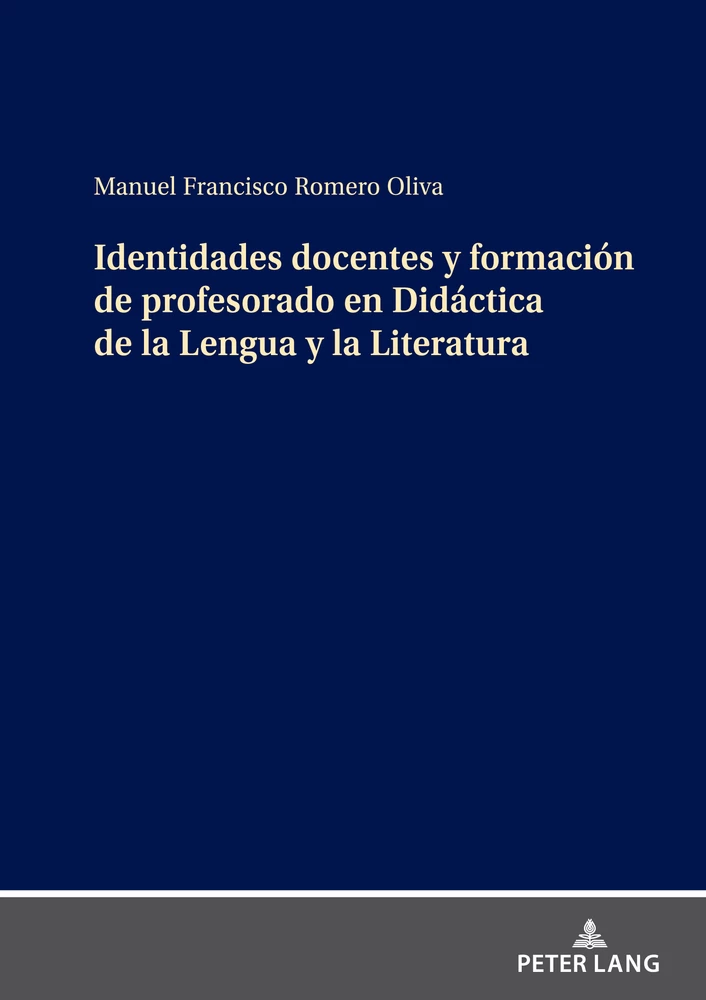
\includegraphics[width=0.5\textwidth]{Fig1.png}
 \caption*{\fullcite{romero_oliva_identidades_2022}.}
 %\caption{\fullcite{nascimento_formacao_2019}.}
 \label{fig01}
% \source{fonte.}
\end{figure}


En el año 2022 Manuel Francisco Romero Oliva, profesor del Departamento de Didáctica de la Lengua y de la Literatura de la Universidad de Cádiz, publica \textit{Identidades docentes y formación de profesorado en Didáctica de la Lengua y la Literatura}. En este sentido, este libro se presenta como el culmen de la ideología educativa del profesor Romero Oliva, quien se ha perfilado estos últimos años como miembro indispensable del área, contando con una amplia trayectoria docente e investigadora que avalan este hecho. Así, el autor centra la obra en la reflexión e investigación sobre la docencia en las asignaturas específicas del Máster Universitario de Formación de Profesorado de Educación Secundaria, Bachillerato, F.P. Y E.O.I. (de ahora en adelante, MAES).

Como adelanta Trujillo en la presentación, “el libro […] es un acto de amor a la democracia, a la convivencia, a una sociedad en paz que utiliza las lenguas (¡y la literatura!) para buscar la felicidad compartida y el bienestar de todos y para todos” (p.14).  Esta declaración de intenciones que vislumbra Trujillo es el hilo conductor de la obra, desde la que se va descubriendo, como si se tratara de un papel de calco, de manera precisa y preciosa, esa \textit{ideología docente} en la que hace hincapié Romero Oliva en todo momento y que ya se pone de manifiesto desde el prólogo.

Este volumen se puede dividir externamente en tres bloques. En primer lugar, se hace un recorrido por la fundamentación científica y curricular de la Didáctica de la Lengua y de la Literatura (más adelante, DLL). En segundo lugar, el autor desgrana lo que él llama \textit{ánforas formativas} para el área. La tercera parte culmina con la reflexión sobre el tercer espacio educativo. A continuación, se irán describiendo los tres bloques.

El primer bloque se titula “Fundamentación científica y curricular de la Didáctica de la Lengua y de la Literatura”. Para ilustrarlo, se divide en tres capítulos. En el primero, “Entre la epistemología y la identidad de la Lengua y la literatura”, se hace un recorrido por el área de la DLL. En este recorrido se hace hincapié no solo en los albores de la DLL, sino también sobre otras disciplinas y áreas que confluyen con esta. Así, tras este análisis, se sitúa a la DLL desde dos perspectivas: una teórica y otra metodológica que “representa las bases de fundamentación de nuestra planificación para la acción docente” (p. 53). Al hilo de esta perspectiva metodológica, resulta interesante el análisis que se realiza sobre la perspectiva educativa y social de la DLL, que se define como un área ya bien consolidada y específica y recogiendo líneas de investigación que trabajen para la sociedad y para la mejora de la acción docente.

El segundo capítulo, “Hacia una transposición didáctica contextualizada de la Didáctica de la Lengua y la Literatura”, se centra en dos cuestiones pertinentes: por un lado, se hace hincapié en “impregnar el currículo de la epistemología del área y diseñar desde la comprensión de la enseñanza de la lengua y la literatura” (p.99) en la que se presenta esa relación indivisible entre área y currículo, siempre desde la perspectiva del MAES, en varios aspectos: los objetivos de enseñanza y etapa; las competencias; los contenidos y destrezas el relación con el logro de objetivos; la ordenación de contenidos en relación con las asignatura y cursos; la metodología didáctica; y la evaluación. El capítulo acaba con “una propuesta de actualización y autentificación del currículo” que se basa en la formación de lectores. Un punto muy interesante de esta propuesta es el decálogo que se ofrece y que “puede servir de referencia para intentar crear una cultura de centro que apueste por la lectura” (p. 148).

Tras esta declaración de intenciones, nos adentramos en el tercer capítulo y último de este primer bloque, “Un punto de arranque: el viaje iniciático hacia las ciencias sociales en el ámbito de la educación”. Este capítulo se centra en ese \textit{viaje iniciático} que supone cursar el MAES, desde la perspectiva de los estudiantes. Ese viaje que es la formación inicial supone el ejercicio de madurez de confrontar las expectativas con la realidad docente y cómo se analiza desde las creencias y vivencias previas a la búsqueda de la identidad docente. De esta manera, se reflexiona, en las últimas páginas del capítulo, sobre esa confrontación entre la realidad “donde confluyen las enseñanzas para ejercer la docencia y las prácticas en los centros educativos” (p.179) y el deseo “de atender a las demandas que la sociedad nos exige para afrontar una educación sostenible en la enseñanza de lenguas y la literatura” que supone cursar el MAES. Este panorama nos introduce el segundo bloque del proyecto centrado en dos vías: la educación lingüística “desde una formación lingüística y comunicativa del docente” (p.180) y la educación literaria “desde la formación lectora y literaria del docente” (p.180).

Como se ha adelantado, el segundo bloque introducido por el capítulo cuatro, “Ánforas formativas y nudos gordianos ante una educación lingüística y literaria”, supone el epicentro de la \textit{ideología docente} del autor, además de deslumbrar su identidad docente con respecto al área. Como se adelanta en el título del capítulo, esta identidad e ideología versan sobre dos ejes: por un lado, las ánforas “como recipientes donde se aloja el conocimiento, presentados en forma de propuestas didácticas para afrontar la reflexión epistemológica de los contenidos que son objeto de enseñanza” (p.185); y, por otro lado, los nudos gordianos, “como retos pendientes de solucionar en el desarrollo de los contenidos en la escuela”, confrontando modelos de aprendizaje como un proceso de autocrítica docente con respecto al marco de la DLL. Estos nudos gordianos son objeto de las propuestas de las ánforas: hábitos lectores y prácticas sociales; comprensión lectora; oralidad; escritura y ortografía; y la gramática. En este sentido, se sitúa a la formación inicial como un espacio de debate de estos nudos para esa identidad docente.

Las ánforas que se proponen son cinco y todas ellas siguen la misma pauta para su actuación: contexto; contenidos, competencias y resultados de aprendizaje; tópico desencadenante; actividades formativas; evidencia formativa; decálogo formativo; y lecturas y materiales para la reflexión. Se describen, a continuación, cada una de las ánforas, mediante este proceso pautado, en las que todas ellas tienen como otro núcleo común la democratización de la identidad docente.

En la primera, “Planificación de la lengua y la literatura desde la comprensión del currículo”, el contexto se centra en la comprensión de la enseñanza, tomando como tópico desencadenante las creencias y actitudes de nuestra lengua oral. La evidencia formativa es la planificación del texto en contexto. El decálogo formativo versa sobre la planificación desde la reflexión docente.  

La segunda ánfora, “Comunicación oral y habilidades lingüísticas”, se plantea como la búsqueda de un método de la oralidad en la escuela. Se propone el aula como un espacio de interacción y se atienden problemas como la confrontación entre el discurso coloquial y formal. En este sentido, se recomienda la oralidad bajo dos vías de actuación: para la gestión de la interacción social del aula y como aprendizaje para mejorar en lo académico y personal. Los contenidos, competencias y resultados de aprendizaje se centran en la alfabetización de la lectura y la escritura y el tópico desencadenante es una reflexión sobre las creencias y actitudes de nuestra lengua oral. Como evidencia formativa también se propone la planificación del texto en contexto y el decálogo formativo se centra en la didáctica de la comunicación oral.

La tercera ánfora trata de la comunicación escrita y las habilidades lingüísticas. En esta, se hace hincapié en los enfoques intensivos y extensivos y la lectura y escritura en la sociedad actual. Los contenidos, competencias y resultados de aprendizaje se centran en la alfabetización de la lectura y la escritura y el tópico desencadenante es la lectura y la escritura para la escuela y para la vida. Como evidencia formativa también se propone la planificación del texto en contexto y el decálogo formativo se centra en la didáctica de la comunicación escrita.

La cuarta ánfora se corresponde con “Del conocimiento de la lengua a la formación lingüística”. En ella, se hace un recorrido por el paradigma en la enseñanza de la lengua, los libros de texto y la didáctica del texto y la gramática. Los contenidos, competencias y resultados de aprendizaje se centran en la funcionalidad de la gramática y el tópico desencadenante es la gramática, el currículo y la enseñanza de la lengua. Como evidencia formativa se propone la planificación desde la didáctica del texto y el decálogo formativo se centra en la didáctica del texto.

La quinta y última ánfora recoge “La formación lectora y literaria” y se centra en el contexto educacional y las referencias para una formación lectoliteraria. En este sentido, se proponen tres vías para su consecución: desde los libros de no ficción; desde la literatura infantil y juvenil; y desde la lectura de los clásicos. Los contenidos, competencias y resultados de aprendizaje se centran en el acercamiento de la literatura al aula y el tópico desencadenante es la actualización y autentificación del currículo. La evidencia formativa se ejemplifica con el taller literario y el decálogo formativo se centra en la formación lectora y literaria.

Este proyecto se culmina con el último bloque a modo de epílogo “La creación de un tercer espacio educativo: uniendo sinergias formativas”. En él se pone de manifiesto el problema de desconexión que se ha sufrido (y sufre) entre escuela y universidad y que se advierte, sobre todo, en el periodo de prácticas del alumnado en formación inicial del MAES. Para ello se recomiendan dos soluciones viables: la creación de ese tercer espacio, donde ambas puedan tenderse la mano, reflexionar y trabajar juntas para seguir construyendo, por supuesto, a través de la delimitación de roles en los agentes implicados del prácticum.

Tras el análisis de la obra, se puede constatar que \textit{Identidades docentes y formación de profesorado en Didáctica de la Lengua y la Literatura} supone un volumen de referencia para el área de la DLL, en este mundo donde el quehacer docente universitario se encuentra siempre en el punto de mira, Romero Oliva nos recuerda que, en palabras de Bell Hooks,

\begin{quote}
    el placer de enseñar es un acto de resistencia que contrarresta el aburrimiento, la falta de interés y la apatía apabullantes que con tanta frecuencia caracterizan el modo en el que profesores y estudiantes viven la enseñanza y el aprendizaje, la experiencia del aula \cite[p. 32]{hooks_ensenar_2021}.
\end{quote}

\printbibliography\label{sec-bib}
% if the text is not in Portuguese, it might be necessary to use the code below instead to print the correct ABNT abbreviations [s.n.], [s.l.]
%\begin{portuguese}
%\printbibliography[title={Bibliography}]
%\end{portuguese}


\end{document}